\section{RT0 三维外场算例}
\label{chapter:07}

% block-id: 07.rt0.p1
\hypertarget{07.rt0.p1}{}
算例为 1×1×2 mm 均质铜长方体，频率 200 kHz，外加 Bz=1 mT RMS，净输运电流为零。三分量电流以面通量自由度表示，分别检查连续性、端口约束和外场功率。采用 q=14 积分时，8192、16000、27648 单元的损耗为 0.927463、0.933539、0.936927 mW；连续两次细化变化为 0.655090\% 和 0.362916\%，低于 1\% 目标。末档提高至 q=18 后，损耗与复面通量的相对变化分别为 1.55×10⁻⁸ 和 1.39×10⁻⁸，低于 0.1\% 积分目标，见 图~\ref{fig:rt0_spatial}。

% block-id: 07.rt0.p2
\hypertarget{07.rt0.p2}{}
切面和矢量图分别见 图~\ref{fig:rt0_sections}、图~\ref{fig:rt0_vectors}，均由保存的面通量恢复。单元中心电流由相对两面的通量平均后除以面面积得到；单元平均损耗密度采用完整 RT0 局部重叠积分，因此包含单元内电流变化。箭头表示零相位时刻电流的实部，并采用统一长度比例，色标表示复 RMS 范数。切面位置和矢量抽样对应图中标注，体积分则使用全部单元。

% block-id: 07.rt0.p3
\hypertarget{07.rt0.p3}{}
各档记录的 GMRES 迭代次数为 35，真残差满足 10⁻¹¹ 目标。空间与积分比较共同支持固定外场长方体的数值结论，适用范围尚未扩展至曲线 Litz 掩膜、独立边界通量验证和实际输运端接。q=18 原摘要中的缺失指标与失败状态、基于 CSV 的后处理验收，以及致密和矩阵自由实现的资源记录分别列入来源资料，以保持求解和数据解释的对应关系。

% block-id: 07.figure.rt0_sections
\hypertarget{07.figure.rt0_sections}{}
\begin{figure}[!htbp]
\centering
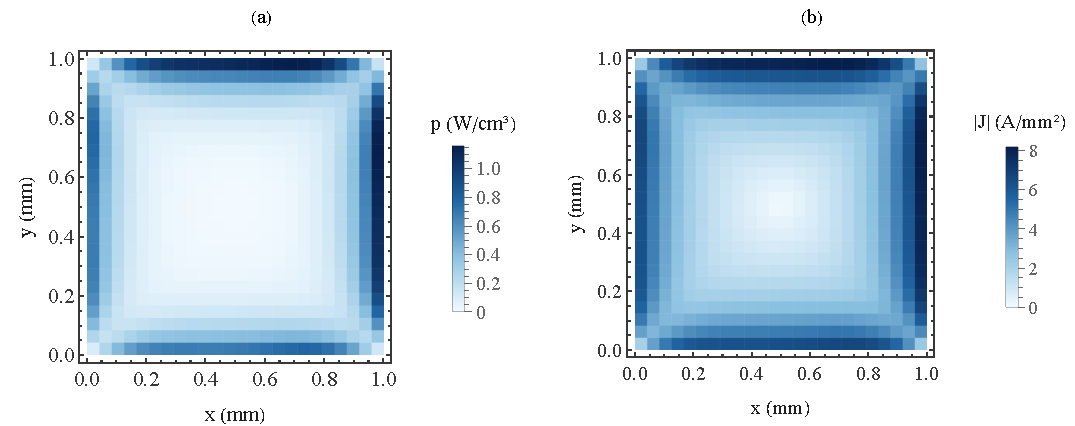
\includegraphics[width=\linewidth,height=.72\textheight,keepaspectratio]{../../assets/zh-CN/rt0_sections.pdf}
\caption{RT0 外场电流与损耗切面。 铜长方体为 1×1×2 mm，200 kHz、1 mT RMS 外场、零净输运。 (a) 单元平均损耗密度；(b) 复 RMS 电流范数。 电流由相对面通量恢复，单元平均损耗采用 RT0 重叠积分。切面位置和色标对应归档的重构定义。}
\label{fig:rt0_sections}
\end{figure}

% block-id: 07.figure.rt0_vectors
\hypertarget{07.figure.rt0_vectors}{}
\begin{figure}[!htbp]
\centering
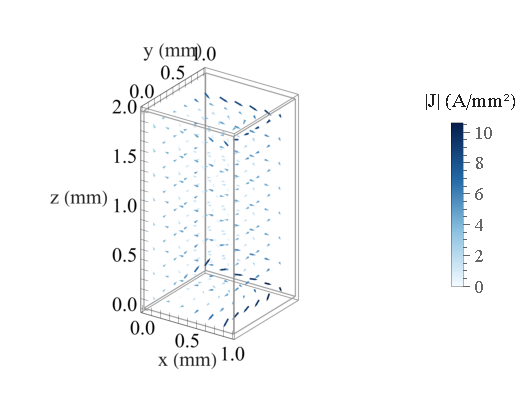
\includegraphics[width=\linewidth,height=.72\textheight,keepaspectratio]{../../assets/zh-CN/rt0_vectors.pdf}
\caption{RT0 重构电流三维矢量。 铜长方体为 1×1×2 mm，200 kHz、1 mT RMS 外场、零净输运。 箭头为固定相位的实部，色标为复 RMS 范数。 矢量采用固定比例与稀疏单元采样。单元与面通量身份在保存的重构数据中对应。}
\label{fig:rt0_vectors}
\end{figure}

% block-id: 07.figure.rt0_spatial
\hypertarget{07.figure.rt0_spatial}{}
\begin{figure}[!htbp]
\centering
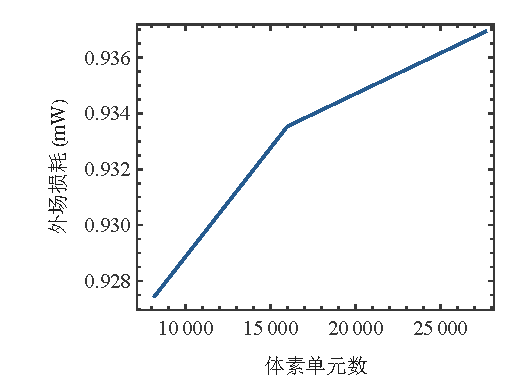
\includegraphics[width=\linewidth,height=.72\textheight,keepaspectratio]{../../assets/zh-CN/rt0_spatial.pdf}
\caption{RT0 空间与积分对照。 铜长方体为 1×1×2 mm，200 kHz、1 mT RMS 外场、零净输运。 q14 空间序列与末档 q18 对照使用相同外场工况。 空间序列为 8192、16000、27648 单元。积分对照在最终成功网格上进行。}
\label{fig:rt0_spatial}
\end{figure}
